\documentclass[a4paper]{article}

\usepackage{tikz}
\usepackage{amsmath}

\newcommand{\entropy}[1]{\mathcal{H}(#1)}

\begin{document}

Suppose we have a program \textit{P}, which takes a set of inputs \textit{I}.
We select a path in the program, at the end of which we observe the set of
outputs \textit{O}. This singular path can have some branches along it, which
will lead certain inputs from \textit{I} along them.

\begin{center}
    \begin{tikzpicture}
        [inner sep=2mm,
         io/.style={rectangle, draw, font=\itshape}]
        \node (input)  at (-5, 0)[io] {I};
        \node (output) at ( 5, 0)[io] {O};
        \draw [->] (input.east) -- (output.west);
        \draw [dashed, ->] (-3, 0) -- (-1, 0.5);
        \draw [dashed, ->] (-1, 0) -- (-0.5, -0.5);
        \draw [dashed, ->] ( 2, 0) -- ( 3, -0.5);
    \end{tikzpicture}
\end{center}

We select \(I_1 \subset I\), such that \textbf{all} inputs from \(I_1\) will
yield a corresponding value in \(O\). This is the reverse image of \(O\) on
\(I\) (I think).

\begin{center}
    \begin{tikzpicture}
        [inner sep=2mm,
         io/.style={rectangle, draw, font=\itshape}]
        \node (input)  at (-5, 0)[io] {$I_1$};
        \node (output) at ( 5, 0)[io] {O};
        \draw [->] (input.east) -- (output.west);
    \end{tikzpicture}
\end{center}

We can then compute the entropy of \(I_1\) and \(O\). We assume \(I_1\) has a
distribution, such as a normal distribution, and we compute the induced
distribution of \(O\) (something something, this is where I'm lost). With
these distributions, we can compute the entropy, by applying the formulas.

\begin{center}
    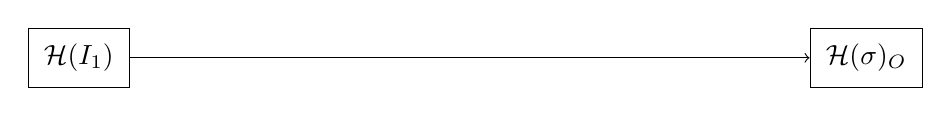
\begin{tikzpicture}
        [inner sep=2mm,
         io/.style={rectangle, draw, font=\itshape}]
         \node (input)  at (-5, 0)[io] {$\entropy{I_1}$};
         \node (output) at ( 5, 0)[io] {$\entropy\sigma_O$};
        \draw [->] (input.east) -- (output.west);
    \end{tikzpicture}
\end{center}

Having computed the entropies, we can now deduce the uncertainty coefficient
(aka Theil's \(U\)), and then compare it to what we obtain be performing
instruction by instruction multiplication, to validate our assumption.

\begin{center}
    \begin{equation*}
        U * \entropy{I_1} = \entropy{\sigma_O}
    \end{equation*}
\end{center}

\end{document}

